% \documentclass[handout]{beamer} %"handout" serveix per a treure els \pause
\documentclass{beamer} %"handout" serveix per a treure els \pause
\usepackage{preamble}
\usepackage{../preamble_bib}

\addbibresource{references.bib} % add bibliography file.

\usetheme{Copenhagen}
\usecolortheme{seahorse}


%gets rid of bottom navigation bars
\setbeamertemplate{footline}[frame number]{}

%gets rid of bottom navigation symbols
\setbeamertemplate{navigation symbols}{}

% remove section and subsection from header
\setbeamertemplate{headline}{}

% set right and left margins
\setbeamersize{text margin left=10pt,text margin right=10pt}

\title{2D Turbulence spreading}
\author{
	Víctor Ballester\texorpdfstring{\vspace{0.45cm}\\}{}{\small Supervisors: Alexandros Alexakis (ENS)\texorpdfstring{\\}{}
\hspace{1.5cm} Emmanuel Dormy (ENS)}}
% \institute{Departament de Matemàtiques\\Facultat de Ciències}
\date{May 24, 2024}

\begin{document}
\thispagestyle{empty}
\frame[noframenumbering]{\titlepage}
% set the counter to 0
\setcounter{framenumber}{0}
\begin{frame}{Navier-Stokes equations}
	\textcolor{\mycolorhighlight}{Navier-Stokes equations} describe the motion of fluids. For an \emph{incompressible fluid} (i.e.\ volume-preserving), they are given by:
	\begin{align*}
		\partial_t \mathbf{u} + (\mathbf{u} \cdot \grad) \mathbf{u} & = -\frac{1}{\rho}\grad p + \nu \laplacian \mathbf{u} + \mathbf{f} \\
		\divp \mathbf{u}                                            & = 0
	\end{align*}
	where $\mathbf{u}(\mathbf{x},t)$ is the velocity field, $p(\mathbf{x},t)$ is the pressure, $\rho(\mathbf{x},t)$ is the density, $\nu$ is the kinematic viscosity, and $\mathbf{f}(\mathbf{x},t)$ is an external force.

	% \begin{minipage}{0.68\textwidth}
	% 	\vspace{-0.5cm}
	% 	These equations can be simplified by adimensionalizing the variables:
	% 	\begin{align*}
	% 		\partial_t \mathbf{u} + (\mathbf{u} \cdot \grad) \mathbf{u} & = -\grad p + \frac{1}{\Re}\laplacian \mathbf{u} + \mathbf{f} \\
	% 		\divp \mathbf{u}                                            & = 0
	% 	\end{align*}
	% 	where $\Re=\frac{UL}{\nu}$ is the \textcolor{\mycolorhighlight}{Reynolds number}, $U$ is a characteristic velocity and $L$ is a characteristic length.
	% \end{minipage}
	% \hfill
	% \begin{minipage}{0.3\textwidth}
	% 	\begin{figure}
	% 		\centering
	% 		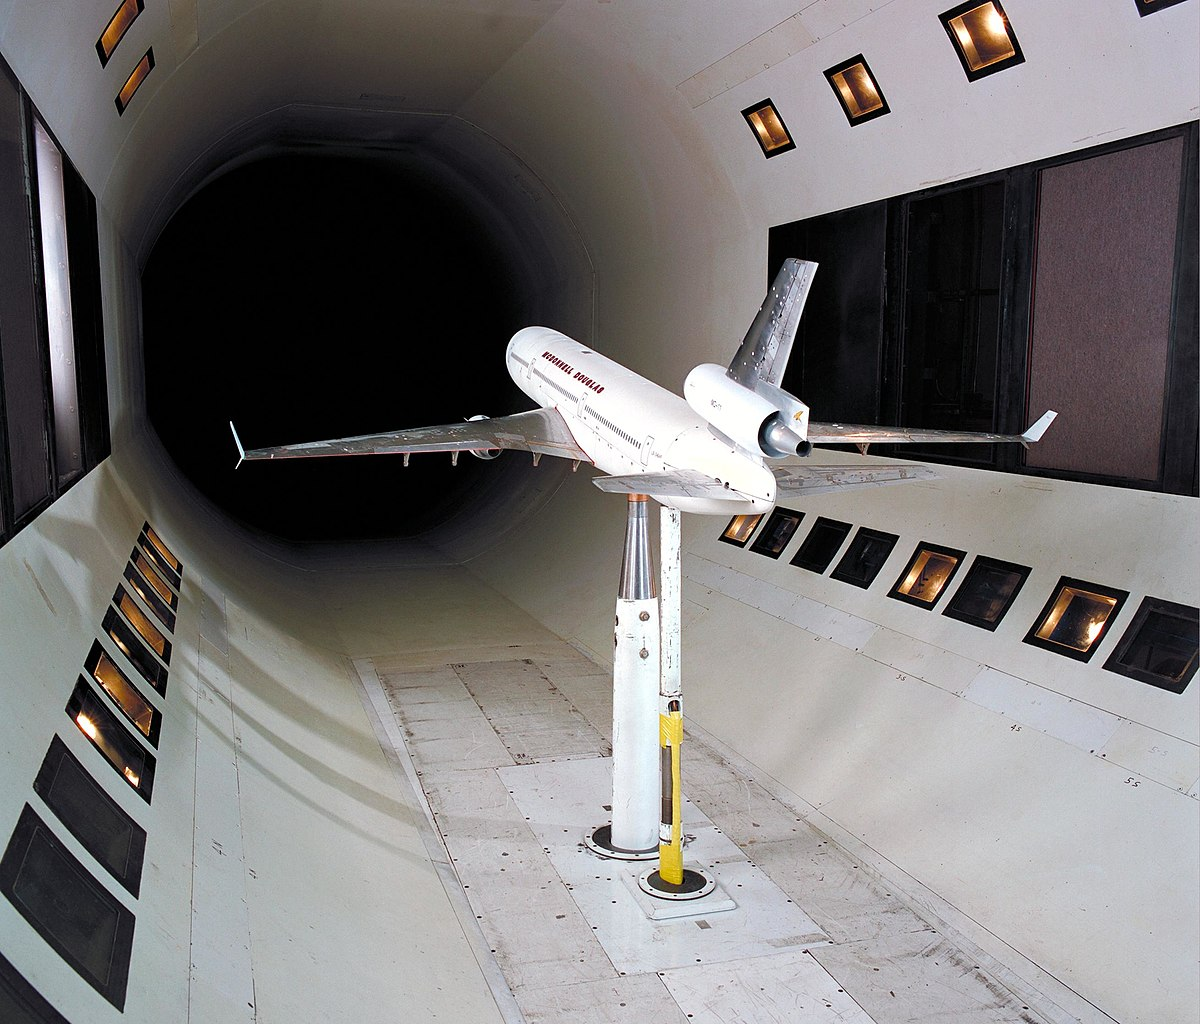
\includegraphics[width=\textwidth]{images/windtunnel.jpg}
	% 		\caption{Model of an airplane in a wind tunnel}
	% 	\end{figure}
	% \end{minipage}

	% % \vspace{-1cm}
\end{frame}
\begin{frame}{What is turbulence?}
	There is no universally accepted definition of turbulence, but people agree on:
	\begin{itemize}
		\item In a turbulent flow, the velocity field is chaotic (in the sense of dynamical systems).
		\item There is wide range of scales involved in the flow.
	\end{itemize}

	\begin{minipage}{0.48\textwidth}
		The onset of turbulence is usually characterized by the \textcolor{\mycolorhighlight}{Reynolds number} (Re), which measures the ratio of inertial forces to viscous forces.
	\end{minipage}\hfill
	\begin{minipage}{0.48\textwidth}
		\begin{figure}
			\centering
			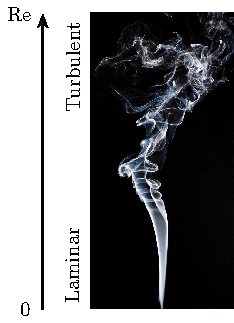
\includegraphics[width=0.48\textwidth]{images/arrowRe.pdf}
			\caption{Smoke from a cigarette.}
		\end{figure}
	\end{minipage}
\end{frame}
\begin{frame}{2D turbulence vs 3D turbulence}
	They are very different! In a nutshell:
	\begin{itemize}
		\item In 3D, energy injected at large scales transfers to small scales.
		\item In 2D, energy injected at intermediate scales transfers to large scales.
	\end{itemize}

	\vspace{0.3cm}
	\begin{figure}
		\centering
		\href{./videos/condensation_small_fast.mp4}{
			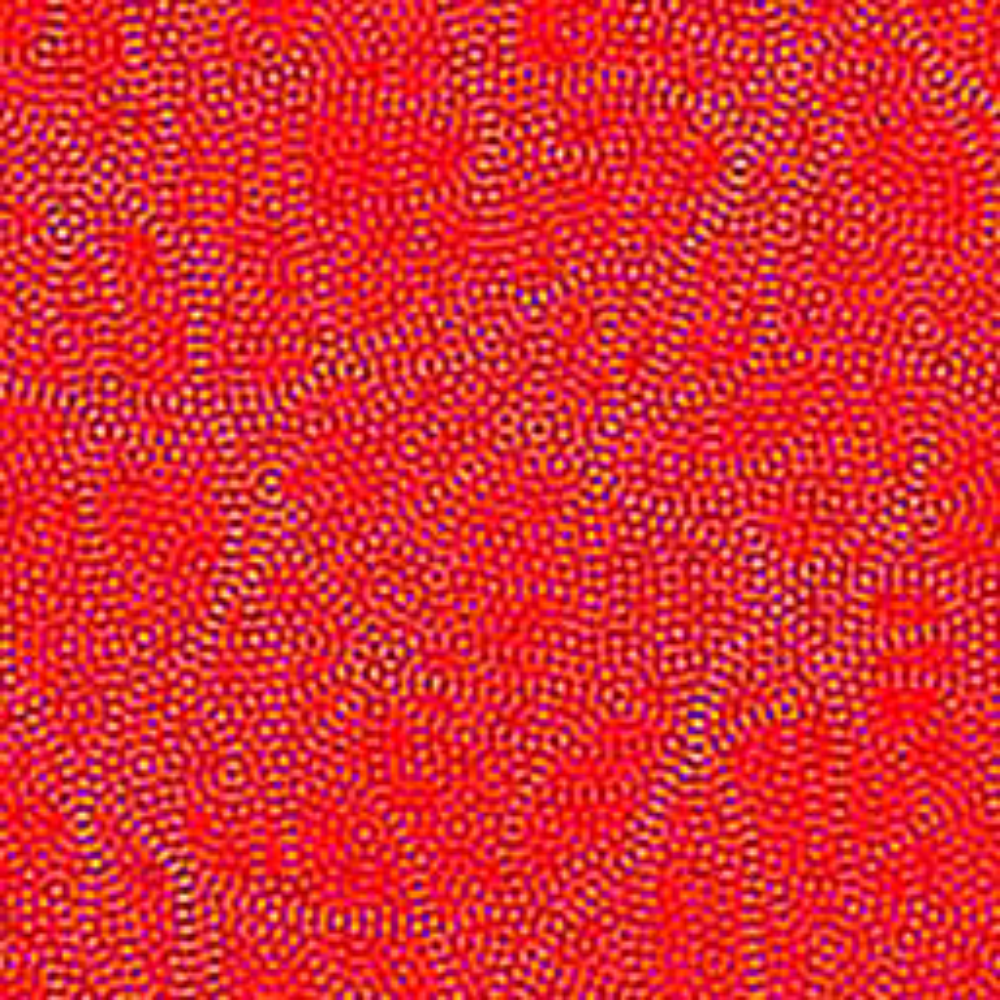
\includegraphics[width=0.3\textwidth]{images/condensation_small_fast-0.png}
		}
		\caption{2D turbulence without forcing}
	\end{figure}
\end{frame}
\begin{frame}{Our problem}
	We consider a periodic box in which we constantly inject energy randomly in the middle. We want to study how this energy spreads in the box.
	\begin{itemize}
		\item Will the energy spread to the whole box?
		\item If so, how long will it take? Which distribution (as a function of the distance to the center) will it follow?
	\end{itemize}
	\begin{figure}
		\centering
		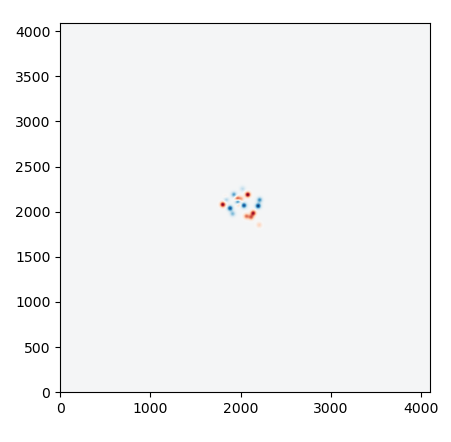
\includegraphics[width=0.3\textwidth]{images/FlowD_fw.002.png}
		\caption{Vorticity ($\curl \vf{u}$) forcing}
	\end{figure}
\end{frame}
\begin{frame}{State-of-the-art and progress}
	\begin{itemize}
		\item In some 3D cases, the energy dissipates before reaching the boundaries of the box \cite{alexakis}.
		\item In 2D\ldots\ seems to spread to the whole box!!
	\end{itemize}
	We would like to see that even decreasing the perturbation region, the vortices fill the whole box as $t\to\infty$ and $\Re\to\infty$.

	\vspace{0.3cm}
	\begin{figure}
		\centering
		\href{./videos/Re64.mp4}{
			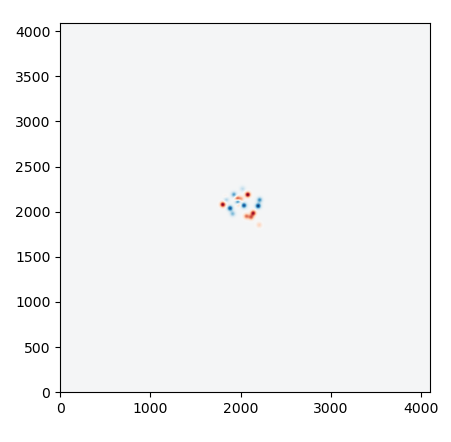
\includegraphics[width=0.3\textwidth]{images/FlowD_fw.002.png}
		}
		\caption{2D turbulence}
	\end{figure}
\end{frame}
\begin{frame}{Post-motivation}
	The main goal is to understand how flows in the atmosphere work.
	\begin{itemize}
		\item In this case, the energy is injected by different local sources, such as storms.
		\item The atmosphere is a very thin 3D domain.
	\end{itemize}
	In these circumstances, will the energy spread to the whole atmosphere? In other words, could a cyclone in Florida affect significantly the weather in Europe?
\end{frame}

\thispagestyle{empty}
\begin{frame}[noframenumbering]{Bibliography}
	\printbibliography
\end{frame}
\end{document}
